% \documentclass[handout]{beamer}
\documentclass{beamer}

\mode<presentation>
{
  \usetheme{ANLBlue}
  % \usefonttheme[onlymath]{serif}
  % \usetheme{Singapore}
  % \usetheme{Warsaw}
  % \usetheme{Malmoe}
  % \useinnertheme{circles}
  % \useoutertheme{infolines}
  % \useinnertheme{rounded}

  \setbeamercovered{transparent=1}
}

\usepackage[english]{babel}
\usepackage[latin1]{inputenc}
\usepackage{alltt,listings,multirow,ulem,siunitx}
\usepackage[absolute,overlay]{textpos}
\TPGrid{1}{1}
\usepackage{pdfpages}
\usepackage{ulem}
\usepackage{multimedia}
\usepackage{multicol}
\newcommand\hmmax{0}
\newcommand\bmmax{0}
\usepackage{bm}
\usepackage{comment}
\usepackage{subcaption}

% font definitions, try \usepackage{ae} instead of the following
% three lines if you don't like this look
\usepackage{mathptmx}
\usepackage[scaled=.90]{helvet}
% \usepackage{courier}
\usepackage[T1]{fontenc}
\usepackage{tikz}
\usetikzlibrary{decorations.pathreplacing}
\usetikzlibrary{shadows,arrows,shapes.misc,shapes.arrows,shapes.multipart,arrows,decorations.pathmorphing,backgrounds,positioning,fit,petri,calc,shadows,chains,matrix}

\newcommand\vvec{\bm v}
\newcommand\bvec{\bm b}
\newcommand\bxk{\bvec_0 \times \kappa_0 \cdot \nabla}
\newcommand\delp{\nabla_\perp}

% \usepackage{pgfpages}
% \pgfpagesuselayout{4 on 1}[a4paper,landscape,border shrink=5mm]

\usepackage{JedMacros}

\newcommand{\timeR}{t_{\mathrm{R}}}
\newcommand{\timeW}{t_{\mathrm{W}}}
\newcommand{\mglevel}{\ensuremath{\ell}}
\newcommand{\mglevelcp}{\ensuremath{\mglevel_{\mathrm{cp}}}}
\newcommand{\mglevelcoarse}{\ensuremath{\mglevel_{\mathrm{coarse}}}}
\newcommand{\mglevelfine}{\ensuremath{\mglevel_{\mathrm{fine}}}}

%solution and residual
\newcommand{\vx}{\ensuremath{x}}
\newcommand{\vc}{\ensuremath{\hat{x}}}
\newcommand{\vr}{\ensuremath{r}}
\newcommand{\vb}{\ensuremath{b}}

%operators
\newcommand{\vA}{\ensuremath{A}}
\newcommand{\vP}{\ensuremath{I_H^h}}
\newcommand{\vS}{\ensuremath{S}}
\newcommand{\vR}{\ensuremath{I_h^H}}
\newcommand{\vI}{\ensuremath{\hat I_h^H}}
\newcommand{\vV}{\ensuremath{\mathbf{V}}}
\newcommand{\vF}{\ensuremath{F}}
\newcommand{\vtau}{\ensuremath{\mathbf{\tau}}}


\title{On adaptive methods in heterogeneous media}
\author{{\bf Jed Brown} \texttt{jed@jedbrown.org} (ANL and CU Boulder) \\
  \quad {\small Collaborators: Mark Adams (LBL), Matt Knepley (UChicago), \\ Dave May (ETH), Laetitia Le Pourhiet (UPMC)}
}

% - Use the \inst command only if there are several affiliations.
% - Keep it simple, no one is interested in your street address.
% \institute
% {
%   Mathematics and Computer Science Division \\ Argonne National Laboratory
% }

\date{National University of Singapore, 2015-02-13 \\[1em]
This talk: \url{http://59A2.org/files/20150213-AdaptHeterogeneous.pdf}}

% This is only inserted into the PDF information catalog. Can be left
% out.
\subject{Talks}


% If you have a file called "university-logo-filename.xxx", where xxx
% is a graphic format that can be processed by latex or pdflatex,
% resp., then you can add a logo as follows:

% \pgfdeclareimage[height=0.5cm]{university-logo}{university-logo-filename}
% \logo{\pgfuseimage{university-logo}}



% Delete this, if you do not want the table of contents to pop up at
% the beginning of each subsection:
% \AtBeginSubsection[]
% {
% \begin{frame}<beamer>
%   \frametitle{Outline}
%   \tableofcontents[currentsection,currentsubsection]
% \end{frame}
% }

% \AtBeginSection[]
% {
%   \begin{frame}<beamer>
%     \frametitle{Outline}
%     \tableofcontents[currentsection]
%   \end{frame}
% }

% If you wish to uncover everything in a step-wise fashion, uncomment
% the following command:

% \beamerdefaultoverlayspecification{<+->}

\begin{document}
\lstset{language=C}
\normalem

\begin{frame}
  \titlepage
\end{frame}

\begin{frame}{Regional scale geodynamic processes}
  \begin{center}
    \includegraphics[width=.85\textwidth]{figures/davemay/WPRegionalGeodynamicsProcesses.png}
  \end{center}
  \begin{columns}
    \begin{column}{0.5\textwidth}
      \begin{itemize}
      \item Buoyancy and topography drive flow
      \item Large variation in length scales
      \item Small scales influence large scales
      \end{itemize}
    \end{column}
    \begin{column}{0.5\textwidth}
      \begin{itemize}
      \item Complex rheology (research)
      \item Material failure (faults)
      \item Post-failure deformation
      \item Thermomechanically coupled
      \end{itemize}
    \end{column}
  \end{columns}
\end{frame}

\begin{frame}{Geology is complicated}
  \begin{columns}
    \begin{column}{0.65\textwidth}
      Zagros Mountains \\
      \includegraphics[width=\textwidth]{figures/davemay/MayZagrosMountains.png} \\
      \vspace{-1ex} {\scriptsize [Yamato et al (2011)]}
% @article{yamato2011dynamic,
%  title={Dynamic constraints on the crustal-scale rheology of the Zagros fold belt, Iran},
%  author={Yamato, Philippe and Kaus, Boris JP and Mouthereau, Fr{\'e}d{\'e}ric and Castelltort, S{\'e}bastien},
%  journal={Geology},
%  volume={39},
%  number={9},
%  pages={815--818},
%  year={2011},
%  publisher={Geological Society of America}
% }
    \end{column}
    \begin{column}{0.35\textwidth}
      European Alps \\
      \includegraphics[width=\textwidth]{figures/davemay/Schmidt2004EuropeanAlps.png}
    \end{column}
  \end{columns}
  \begin{columns}
    \begin{column}{0.6\textwidth}
      \begin{itemize}
      \item Ductile folding
      \item Discontinuous material properties
      \end{itemize}
    \end{column}
    \begin{column}{0.4\textwidth}
      \begin{itemize}
      \item Inherently 3D
      \item Faulting
      \end{itemize}
    \end{column}
  \end{columns}
\end{frame}

\begin{frame}{Continental rifting}
  %\movie[width=\textwidth,height=0.66\textwidth,autostart,poster,showcontrols=false,loop]{Oblique Rifting Video}{dstrong2_truc.mov}
  \movie[width=\textwidth,height=0.66\textwidth,autostart,poster,showcontrols=false,loop]{Rifting Video}{LaetiSC14Rifting.mp4}
\end{frame}

\section{$\tau$-adaptivity}
\begin{frame}[fragile]{Multigrid Preliminaries}
  \begin{figure}
    \centering
    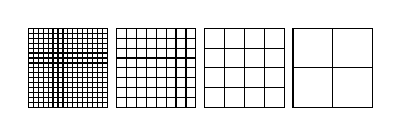
\begin{tikzpicture}
      [>=stealth,
      every node/.style={inner sep=2pt},
      restrict/.style={thick},
      prolong/.style={thick},
      mglevel/.style={rounded rectangle,draw=blue!50!black,fill=blue!20,thick,minimum size=4mm},
      ]
      \begin{scope}\scriptsize
        \newcommand\mgdx{4.0em}
        \newcommand\mgdy{4.0em}
        \newcommand\mgl[1]{(pow(2,#1+1))}
        \newcommand\mgloc[4]{(#1 + #4*\mgdx*#3,#2 + \mgdy*#3)}

        \newcommand\mghx{0.9*\mgdx}
        \newcommand\mghy{0.9*\mgdy}

        \draw[shift=\mgloc{0*\mgdx}{0}{0}{0},
        xstep=\mghy/\mgl{3},
        ystep=\mghy/\mgl{3}]
        (-0.5*\mghy,-0.5*\mghy) grid (0.5*\mghy,0.5*\mghy);

        \draw[shift=\mgloc{1*\mgdx}{0}{0}{0},
        xstep=\mghy/\mgl{2},
        ystep=\mghy/\mgl{2}]
        (-0.5*\mghy,-0.5*\mghy) grid (0.5*\mghy,0.5*\mghy);

        \draw[shift=\mgloc{2*\mgdx}{0}{0}{0},
        xstep=\mghy/\mgl{1},
        ystep=\mghy/\mgl{1}]
        (-0.5*\mghy,-0.5*\mghy) grid (0.5*\mghy,0.5*\mghy);


        \draw[shift=\mgloc{3*\mgdx}{0}{0}{0},
        xstep=\mghy/\mgl{0},
        ystep=\mghy/\mgl{0}]
        (-0.5*\mghy,-0.5*\mghy) grid (0.5*\mghy,0.5*\mghy);
      \end{scope}
    \end{tikzpicture}
    \label{fig:levels}
  \end{figure}
  \textbf{Multigrid} is an $O(n)$ method for solving algebraic problems by defining a hierarchy of scale.
  A multigrid method is constructed from:
  \begin{enumerate}
  \item a sequence of discretizations
    \begin{itemize}
    \item coarser approximations of problem, same or different equations
    \item constructed algebraically or geometrically
    \end{itemize}
  \item intergrid transfer operators
    \begin{itemize}
    \item residual restriction $I_h^H$ (fine to coarse)
    \item state restriction $\hat I_h^H$ (fine to coarse)
    \item partial state interpolation $I_H^h$ (coarse to fine, `prolongation')
    \item state reconstruction $\mathbb{I}_H^h$ (coarse to fine)
    \end{itemize}
  \item Smoothers ($S$)
    \begin{itemize}
    \item correct the high frequency error components
    \item Richardson, Jacobi, Gauss-Seidel, etc.
    \item Gauss-Seidel-Newton or optimization methods
    \item Compatible Monte Carlo, \ldots
    \end{itemize}
  \end{enumerate}
\end{frame}
\input{slides/MG/TauFAS.tex}

\begin{frame}{Model problem: $\pfrak$-Laplacian with slip boundary conditions}
  \begin{itemize}
  \item 2-dimensional model problem for power-law fluid cross-section
    \begin{equation*}
      -\div \big(\abs{\nabla u}^{\pfrak-2} \nabla u \big) - f = 0, \qquad 1 \le \pfrak \le \infty
    \end{equation*}
    Singular or degenerate when $\nabla u = 0$
  \item Regularized variant
    \begin{gather*}
      -\div (\eta \nabla u) - f = 0 \\
      \eta(\gamma) = (\epsilon^2 + \gamma)^{\frac{\pfrak-2}{2}} \qquad \gamma(u) = \half \abs{\nabla u}^2
    \end{gather*}
  \item Friction boundary condition on one side of domain
    \begin{gather*}
      \nabla u \cdot \bm n + A(x) \abs{u}^{q-1} u = 0
    \end{gather*}
  \end{itemize}
\end{frame}

\begin{frame}{Model problem: $\pfrak$-Laplacian with slip boundary conditions}
  \begin{itemize}
  \item $\pfrak = 1.3$ and $q = 0.2$, checkerboard coefficients $\{10^{-2},1\}$
  \item Friction coefficient $A=0$ in center, 1 at corners
  \end{itemize}
  \begin{columns}
    \begin{column}{0.5\textwidth}
      \only<1>{\includegraphics[width=\textwidth]{figures/MG/ex15-friction/visit0010.png}}
      \only<2>{\includegraphics[width=\textwidth]{figures/MG/ex15-friction/visit0011.png}}
      \only<3>{\includegraphics[width=\textwidth]{figures/MG/ex15-friction/visit0012.png}}
      \only<4>{\includegraphics[width=\textwidth]{figures/MG/ex15-friction/visit0013.png}}
      \only<5>{\includegraphics[width=\textwidth]{figures/MG/ex15-friction/visit0014.png}}
      \only<6>{\includegraphics[width=\textwidth]{figures/MG/ex15-friction/visit0015.png}}
    \end{column}
    \begin{column}{0.5\textwidth}
      \includegraphics[width=\textwidth]{figures/MG/newton-convergence.png}
    \end{column}
  \end{columns}
\end{frame}

\begin{frame}{$\tau$ corrections}
  \begin{figure}
  \centering
  \begin{subfigure}[b]{0.18\textwidth}
    \includegraphics[width=\textwidth]{figures/MG/ElasticityCompressTrim}
    %\caption{Initial solution.}\label{fig:elast-initial}
  \end{subfigure} ~
  \begin{subfigure}[b]{0.18\textwidth}
    \includegraphics[width=\textwidth]{figures/MG/ElasticityCompressShearTrim}
    %\caption{Increment.}\label{fig:elast-increment}
  \end{subfigure} ~
  \begin{subfigure}[b]{0.28\textwidth}
    \includegraphics[width=\textwidth]{figures/MG/ElasticityCompressErrorNoTauTrim}
    %\caption{Smoothed error without $\tau$.}\label{fig:elast-error-notau}
  \end{subfigure} ~
  \begin{subfigure}[b]{0.28\textwidth}
    \includegraphics[width=\textwidth]{figures/MG/ElasticityCompressErrorTauTrim}
    %\caption{Smoothed error with $\tau$.}\label{fig:elast-error-tau}
  \end{subfigure}
  \begin{itemize}
  \item Plane strain elasticity, $E=1000,\nu=0.4$ inclusions in $E=1,\nu=0.2$ material, coarsen by $3^2$.
  \item Solve initial problem everywhere and compute $\tau_h^H = A^H \hat I_h^H u^h - I_h^H A^h u^h$
  \item Change boundary conditions and solve FAS coarse problem
    \begin{equation*}
      N^H \acute u^H = \underbrace{I_h^H \acute f^h}_{\acute f^H} + \underbrace{N^H \hat I_h^H \tilde u^h - I_h^H N^h \tilde u^h}_{\tau_h^H}
    \end{equation*}
  \item Prolong, post-smooth, compute error $e^h = \acute u^h - (N^h)^{-1} \acute f^h$
  \item<2> \alert{Coarse grid \emph{with $\tau$} is nearly $10\times$ better accuracy}
  \end{itemize}
  % \caption{Plane strain elasticity, $E=1000,\nu=0.4$ inclusions in $E=1,\nu=0.2$ material.  2-level multigrid with coarsening factor of $3^2$.
  %   Panes (a) and (b) show the deformed body colored by strain.
  %   The initial problem of compression by 0.2 from the right is solved (a) and $\tau = A^H \hat I_h^H u^h - I_h^H A^h u^h$ is computed.
  %   Then a shear increment of 0.1 in the $y$ direction is added to the boundary condition, and the coarse-level problem is resolved, interpolated to the fine-grid, and a post-smoother is applied.
  %   When the coarse problem is solved without a $\tau$ correction (c), the displacement error is nearly $10\times$ larger than when $\tau$ is included in the right hand side of the coarse problem (d).
  % }\label{fig:tau-valid}
  % ./ex49 -mx 90 -my 90 -da_refine_x 3 -da_refine_y 3 -elas_ksp_converged_reason -elas_ksp_rtol 1e-8 -no_view -c_str 3 -sponge_E0 1 -sponge_E1 1e3 -sponge_nu0 0.4 -sponge_nu1 0.2 -sponge_t 3 -sponge_w 9 -u_o vtk:ex49_sol.vts -use_nonsymbc -elas_pc_type mg -elas_pc_mg_levels 2 -elas_pc_mg_galerkin -tau1_o vtk:ex49_tau1.vts -tau2_o vtk:ex49_tau2.vts -taudiff_o vtk:ex49_taudiff.vts -u2_o vtk:ex49_sol2.vts -u2c_o vtk:ex49_sol2c.vts -u3_o vtk:ex49_sol3.vts -u4_o vtk:ex49_sol4.vts -u2err_o vtk:ex49_sol2err.vts -u3err_o vtk:ex49_sol3err.vts -u3c_o vtk:ex49_sol3c.vts -tau3_o vtk:ex49_tau3.vts
\end{figure}
\end{frame}

\begin{frame}{$\tau$ adaptivity: an idea for heterogeneous media}
  \begin{itemize}
  \item Applications with localized nonlinearities
    \begin{itemize}
    \item Subduction, rifting, rupture/fault dynamics
    \item Carbon fiber, biological tissues, fracture
    \item {\bf Phase-field models for fracture}
    \item {\bf Crystal growth in irregular media}
    \end{itemize}
  \item Adaptive methods fail for heterogeneous media
    \begin{itemize}
    \item Rocks are rough, solutions are not ``smooth''
    \item Cannot build accurate coarse space without scale separation
    \end{itemize}
  \item $\tau$ adaptivity
    \begin{itemize}
    \item Fine-grid work needed everywhere at first
    \item Then $\tau$ becomes accurate in nearly-linear regions
    \item Only visit fine grids in ``interesting'' places: active nonlinearity, drastic change of solution
    \end{itemize}
  \end{itemize}
\end{frame}

\begin{frame}{Comparison to nonlinear domain decomposition}
  \begin{itemize}
  \item ASPIN (Additive Schwarz preconditioned inexact Newton) \\
    \begin{itemize}
    \item Cai and Keyes (2003)
    \item More local iterations in strongly nonlinear regions
    \item Each nonlinear iteration only propagates information locally
    \item Many real nonlinearities are activated by long-range forces
      \begin{itemize}
      \item locking in granular media (gravel, granola)
      \item binding in steel fittings, crack propagation
      \end{itemize}
    \item Two-stage algorithm has different load balancing
      \begin{itemize}
      \item Nonlinear subdomain solves
      \item Global linear solve
      \end{itemize}
    \end{itemize}
  \item $\tau$ adaptivity
    \begin{itemize}
    \item Minimum effort to communicate long-range information
    \item Nonlinearity sees effects as accurate as with global fine-grid feedback
    \item Fine-grid work always proportional to ``interesting'' changes
    \end{itemize}
  \end{itemize}
\end{frame}

\input{slides/MG/SmoothingNonlinearProblems.tex}

\subsection{Reducing communication and memory bandwidth}
\begin{frame}{Plan: ruthlessly eliminate communication}
  \begin{itemize}
  \item Eliminate, not ``aggregate and amortize''
  \end{itemize}
  \begin{block}{Why?}
    \begin{itemize}
    \item Enables pruning unnecessary work
    \item More scope for dynamic load balance
    \item Tolerance for high-frequency load imbalance
      \begin{itemize}
      \item From irregular computation or hardware error correction
      \end{itemize}
    \item Local recovery despite global coupling
    \end{itemize}
  \end{block}
  \begin{block}{Requirements}
    \begin{itemize}
    \item Must retain optimal convergence with good constants
    \item Flexible, robust, and debuggable
    \end{itemize}
  \end{block}
\end{frame}
\input{slides/MG/LowComm.tex}
\begin{frame}{Segmental refinement: no horizontal communication}
  \begin{itemize}
  \item Adams, Brown, Knepley, Samtaney, \hyperref{http://arxiv.org/abs/1406.7808}{}{}{arXiv:1406.7808}
  \item 27-point second-order stencil, manufactured analytic solution
  \item 5 SR levels: $16^3$ cells/process local coarse grid
  \item $\text{Overlap} = \text{Base} + (L-\ell) \text{Increment}$
    \begin{itemize}
    \item Implementation requires even number of cells---round down.
    \end{itemize}
  \item FMG with $V(2,2)$ cycles
  \end{itemize}
  \begin{columns}
    \begin{column}{0.4\textwidth}
      \begin{table}\small
        \centering\caption{$\norm{e_{SR}}_\infty / \norm{e_{FMG}}_\infty$}\label{tab:sr-error}
        \begin{tabular}{l rrr}
          \toprule
          & \multicolumn{3}{c}{Base} \\
          Increment & 1 & 2 & 3 \\
          \midrule
          1 & {\color{red} 1.59} & {\color{red} 2.34} & 1.00 \\
          2 & 1.00 & 1.00 & 1.00 \\
          3 & 1.00 & 1.00 & 1.00 \\
          \bottomrule
        \end{tabular}
      \end{table}
    \end{column}
    \begin{column}{0.6\textwidth}
      \includegraphics[width=\textwidth]{figures/MG/weak_scaling_edison-eps-converted-to.pdf}
    \end{column}
  \end{columns}
\end{frame}

\begin{frame}{Reducing memory bandwidth}
  \includegraphics[width=\textwidth]{figures/MG/SRMGWindow}
  \begin{itemize}
  \item Sweep through ``coarse'' grid with moving window
  \item Zoom in on new slab, construct fine grid ``window'' in-cache
  \item Interpolate to new fine grid, apply pipelined smoother ($s$-step)
  \item Compute residual, accumulate restriction of state and residual into coarse grid, expire slab from window
  \end{itemize}
\end{frame}

\begin{frame}{Arithmetic intensity of sweeping visit}
  \begin{itemize}
  \item Assume 3D cell-centered, 7-point stencil
  \item 14 flops/cell for second order interpolation
  \item $\ge 15$ flops/cell for fine-grid residual or point smoother
  \item 2 flops/cell to enforce coarse-grid compatibility
  \item 2 flops/cell for plane restriction
  \item assume coarse grid points are reused in cache
  \item Fused visit reads $u^H$ and writes $\hat I_h^H u^h$ and $I_h^H r^h$
  \item Arithmetic Intensity
    \begin{equation}
      \frac{{\overbrace{15}^{\text{interp}}} + {\overbrace{2\cdot (15+2)}^{\text{compatible relaxation}}} + \overbrace{2\cdot 15}^{\text{smooth}} + \overbrace{15}^{\text{residual}} + \overbrace{2}^{\text{restrict}}}{3 \cdot \texttt{sizeof(scalar)} / \underbrace{2^3}_{\text{coarsening}}} \gtrsim 30
    \end{equation}
  \item Still $\gtrsim 10$ with non-compressible fine-grid forcing
  \end{itemize}
\end{frame}

\begin{frame}{Regularity}
  Accuracy depends on operator regularity
  \begin{itemize}
  \item Even with regularity, we can only converge up to discretization error, unless we add a \emph{consistent} fine-grid residual evaluation
  \item Visit fine grid with some overlap, but patches do not agree exactly in overlap
  \item Need decay length for high-frequency error components (those that restrict to zero) that is bounded with respect to grid size
  \item Required overlap $J$ is proportional to the number of cells to cover decay length
  \item Can enrich coarse space along boundary, but causes loss of coarse-grid sparsity
  \item Brandt and Diskin (1994) has two-grid LFA showing $J \lesssim 2$ is sufficient for Laplacian
  \item With $L$ levels, overlap $J(k)$ on level $k$,
    \begin{equation*}
      2J(k) \ge s (L-k+1)
    \end{equation*}
    where $s$ is the smoothness order of the solution or the discretization order (whichever is smaller)
  \end{itemize}
\end{frame}

\begin{frame}{Other uses of segmental refinement}
  \begin{itemize}
  \item Compression of solutions, local decompression, resilience
  \item Transient adjoints
    \begin{itemize}
    \item Adjoint model runs backward-in-time, needs state from solution of forward model
    \item Status quo: hierarchical checkpointing
    \item Memory-constrained and requires computing forward model multiple times
    \item If forward model is stiff, each step has global dependence
    \item Compression via $\tau$-FAS accelerates recomputation, can be local
    \end{itemize}
  \item Visualization and analysis
    \begin{itemize}
    \item Targeted visualization in small part of domain
    \item Interesting features emergent so can't predict where to look
    \end{itemize}
  \end{itemize}
\end{frame}

\begin{frame}{Outlook}
  \begin{itemize}
  \item $\tau$ adaptivity: benefits of AMR without fine-scale smoothness
  \item Coarse-centric restructuring is a major interface change
  \item Nonlinear smoothers (and discretizations)
    \begin{itemize}
    \item Smooth in neighborhood of ``interesting'' fine-scale features
    \item Which discretizations can provide efficient matrix-free smoothers?
    % \item Does there exist an efficient smoother based on element Neumann problems?
    \end{itemize}
  \item Weakening data dependencies enables dynamic load balancing
  \item Reliability of error estimates for refreshing $\tau$
    \begin{itemize}
    \item We want a coarse indicator for whether $\tau$ needs to change
    \item Phase fields can provide such information
    \end{itemize}
  \item Exploit structure or explain why it is not exploitable
  \end{itemize}
\end{frame}

\section{Lesser-known solver techniques}
\begin{frame}{Nonlinear deflation for finding multiple distinct solutions}
  Patrick Farrell, \'Asgeir Birkisson, Simon Funke \hyperref{http://arxiv.org/abs/1410.5620}{}{}{arXiv:1410.5620}
  \begin{itemize}
  \item Find a solution $F(u^*) = 0$
  \item Deflate system using $\eta(u;u^*) = \norm{u - u^*}$ or variants
    \begin{equation*}
      G(u) = \frac{F(u)}{\eta(u;u^*)} = 0
    \end{equation*}
  \item Jacobian has structure
    \begin{equation*}
      \nabla_u G(u) = \frac{\nabla_u F(u)}{\eta(u;u^*)} - \underbrace{\frac{F(u)}{\eta^2(u;u^*)} \eta'(u;u^*)}_{\text{rank 1, dense}}
    \end{equation*}
  \item Apply Jacobian matrix-free, precondition using Woodbury formula
  \item Application to Allen-Cahn, Yamabe, Navier-Stokes, and others
  \item Preconditioning using PETSc's GAMG; number of iterations constant for each solution
  \item Extension to nonlinear eigenproblems?
  \end{itemize}
\end{frame}

\begin{frame}{FAS-EIS for eigenproblems}
  Cohen, Kronik, Brandt, {\it Locally Refined Multigrid Solution of the All-Electron
Kohn-Sham Equation}, 2013; Brandt, {\it Multiscale calculation of many eigenfunctions}, 2003; Livne 2001
  \begin{itemize}
  \item Proposes techniques for fast solution of self-consistent Kohn-Sham
  \item Exact Interpolation Scheme (EIS)
    \begin{itemize}
    \item Adapts coarse basis functions to represent eigenfunctions
    \item Orthogonality preserved by interpolation: $O(N K + K^3)$ or better
    \item Can exploit localization
    \item Related to bootstrap AMG
    \end{itemize}
  \item Multiscale Eigen-Basis
    \begin{itemize}
    \item $K$ eigenvalues in $O(N \log K)$
    \item Transform to/from eigenbasis in $O(N \log K)$
    \item Works in 1D, generalization hard
    \end{itemize}
  \end{itemize}
\end{frame}

\section{What is performance?}
\begin{frame}
  \bigskip
  \begin{center}
    {\LARGE \bf What is performance?}
  \end{center}
  \bigskip
  \begin{itemize}
  \item<2> {\Large {\bf Cost-Accuracy} tradeoff}
  \item<2> {\Large {\bf Versatility} with respect to external requirements}
  \end{itemize}
\end{frame}

\begin{frame}{Work-precision diagram: \emph{de rigueur} in ODE community}
  \begin{center}
    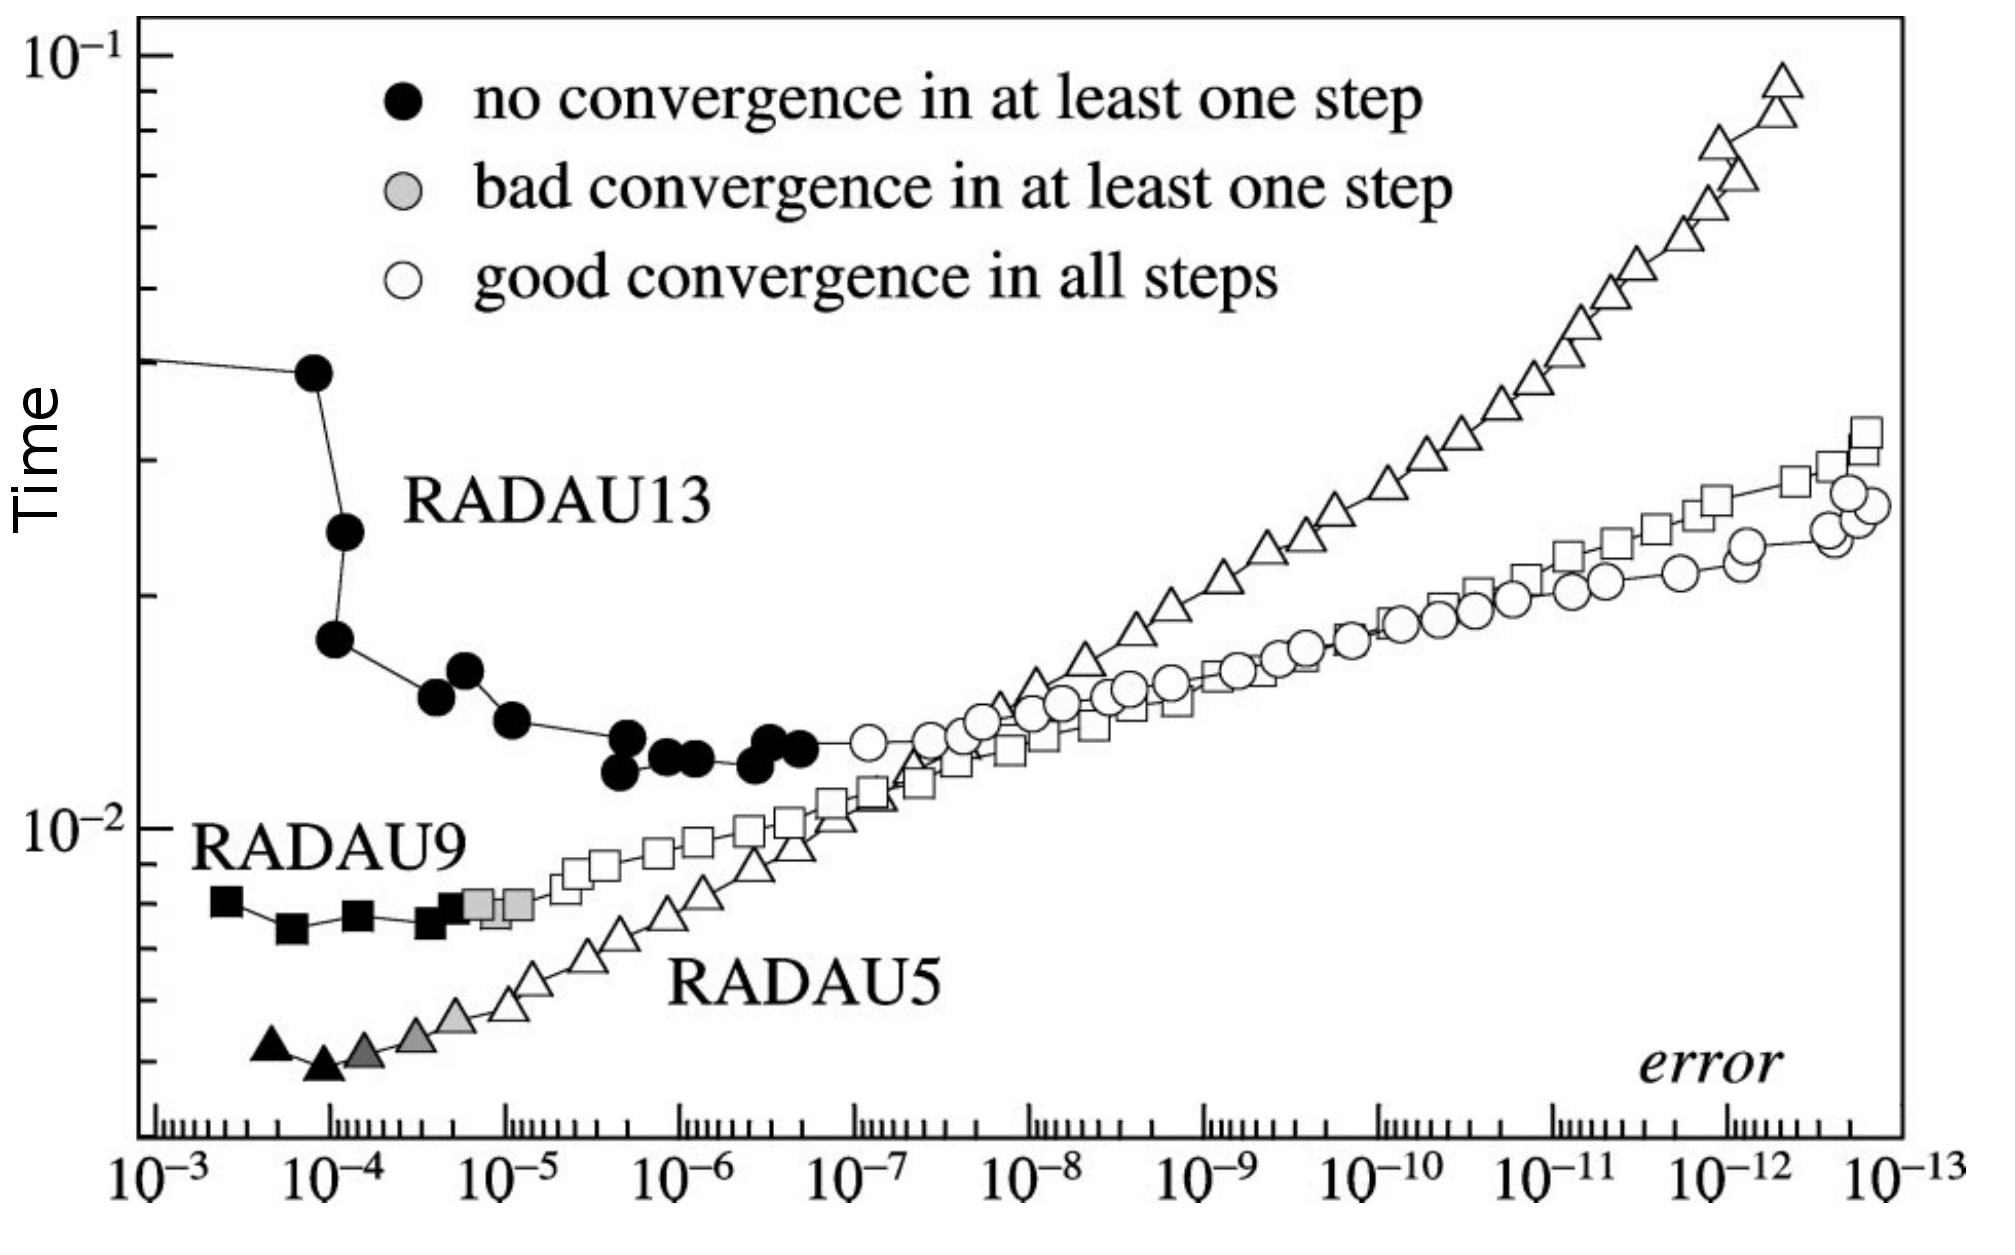
\includegraphics[width=0.8\textwidth]{figures/HairerWanner-WorkPrecision.png}\\
    {\scriptsize [Hairer and Wanner (1999)]}
  \end{center}
  \begin{itemize}
  \item Tests discretization, adaptivity, algebraic solvers, implementation
  \item No reference to number of time steps, number of grid points, etc.
  \end{itemize}
\end{frame}

\begin{frame}{Edison, SuperMUC, Titan}
  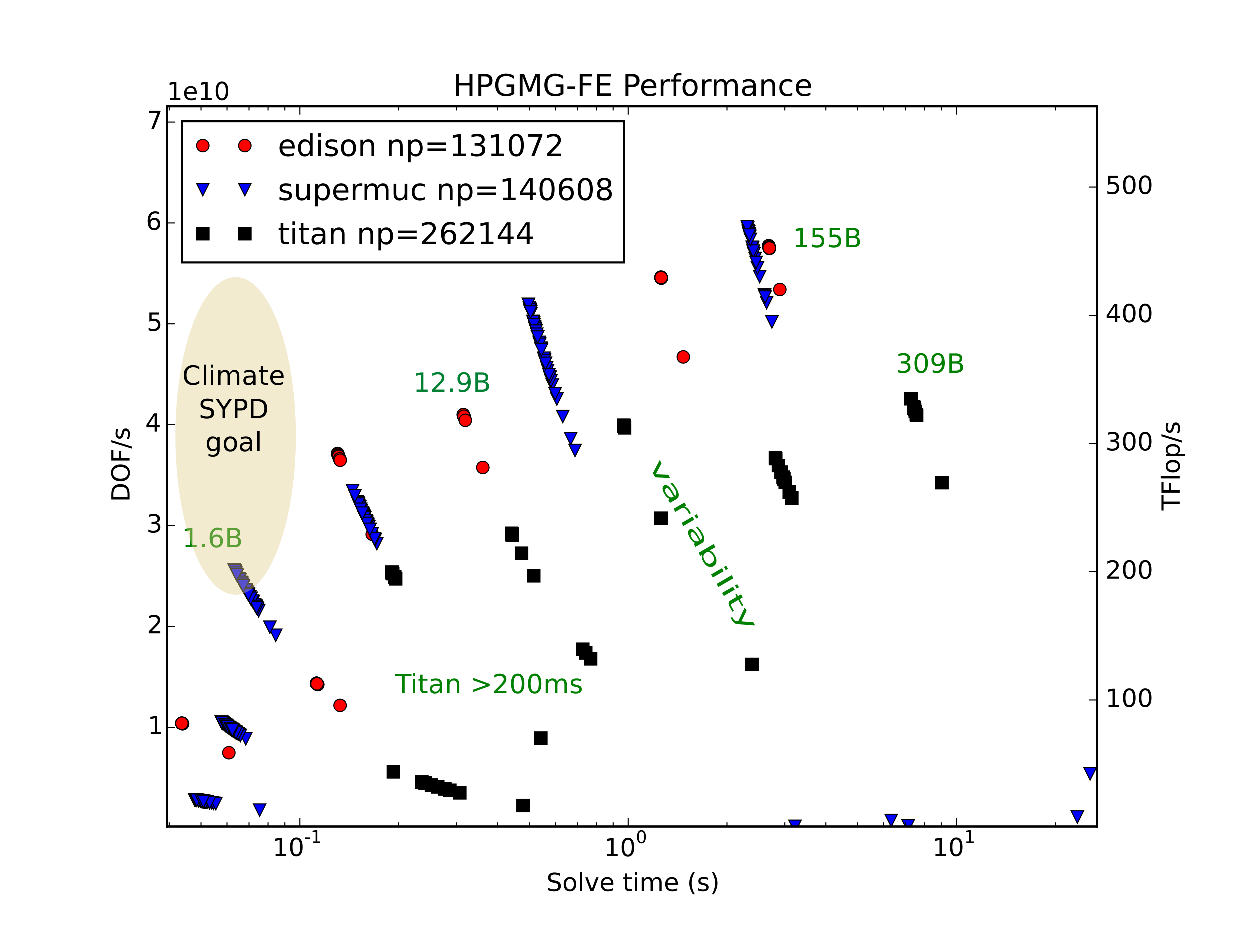
\includegraphics[width=\textwidth]{figures/hpgmg/range-edison-supermuc-titan-ann2.eps}
\end{frame}

\end{document}
